\chapter{Generatieve ontwikkeling en de regeling van de bloei}\label{ch:b2:plant-flowering}

Een chrysantenkweker kan een kas met Kerstmis of met Pasen laten bloeien
door de lampen aan of uit te doen; een wintertarwe die in het voorjaar wordt
gezaaid, bloeit nooit, omdat ze geen kou heeft gehad; een stekelnoot die één
enkele nacht heeft meegemaakt die langer was dan haar kritische lengte, is
tot bloeien vastgelegd, wat er daarna ook gebeurt. Een plant heeft geen
kalender, maar wel klokken, thermometers en lichtmeters, en op grond daarvan
beslist ze eenmaal per jaar om een \omterm{def:b2:plant-meristems:meristem}{meristeem} dat bladeren maakte om te
zetten in een \omterm{def:b2:plant-meristems:meristem}{meristeem} dat een \omterm{def:b2:angiosperm-reproduction:flower}{bloem} zal maken. Dit hoofdstuk volgt die
beslissing van het blad dat de nacht meet tot het \omterm{def:b2:plant-meristems:meristem}{meristeem} dat van
programma verandert, daarna de bouw van de \omterm{def:b2:angiosperm-reproduction:flower}{bloem} volgens een code van
genen, en de omgekeerde overgang aan het andere eind van de cyclus: het \omterm{def:b2:angiosperm-reproduction:seed}{zaad}
dat pas wil kiemen als het te horen krijgt dat het seizoen gunstig is.

\section{De overgang naar de bloei}

\begin{definition}[Bloeiovergang en bloei-inductie]\label{def:b2:plant-flowering:transition}
\index{bloeiovergang}\index{bloei-inductie}\index{bloeiwijzemeristeem}
Een vegetatief \omterm{def:b2:plant-meristems:meristem}{apicaal scheutmeristeem} maakt onbeperkt bladeren met in elke
oksel een knop. Bij de \emph{bloeiovergang} wordt het een
\emph{bloeiwijzemeristeem}, dat schutbladen maakt en, in hun oksels,
\emph{bloemmeristemen}, die elk begrensd zijn: ze maken kelkbladen,
kroonbladen, meeldraden en \omterm{def:b2:angiosperm-reproduction:flower}{vruchtbladen} en stoppen dan. De verandering
wordt in gang gezet door \emph{bloei-inductie} --- een signaal, afkomstig
uit de bladeren of ontstaan in de eigen fysiologie van de plant, dat de
identiteitsgenen van het \omterm{def:b2:plant-meristems:meristem}{meristeem} omschakelt. Eenjarigen bloeien één keer
en sterven; overblijvende planten bloeien elk jaar vanuit sommige
meristemen en houden andere vegetatief. Het tijdstip bepaalt of \omterm{def:b2:plant-life-cycles:heterospory}{stuifmeel}
\omterm{def:b2:plant-life-cycles:heterospory}{stuifmeel} ontmoet, of zaden rijpen vóór de vorst, en of de \omterm{def:b2:angiosperm-reproduction:flower}{bloem} opengaat
wanneer haar bestuiver vliegt: het staat onder sterke selectie, en planten
hebben verschillende manieren ontwikkeld om het seizoen af te lezen.
\end{definition}

\begin{proposition}[Fotoperiodiciteit: de plant meet de nacht]\label{prop:b2:plant-flowering:photoperiod}
\index{fotoperiodiciteit}\index{korte-dagplant}\index{lange-dagplant}\index{fytochroom}
Veel planten bloeien als reactie op de daglengte. \emph{\omterm{prop:b2:plant-flowering:photoperiod}{Korte-dagplanten}}
(chrysant, sojaboon, rijst, stekelnoot) bloeien wanneer de dag korter is dan
een kritische lengte --- in de herfst of het voorjaar;
\emph{\omterm{prop:b2:plant-flowering:photoperiod}{lange-dagplanten}} (spinazie, tarwe, klaver, \emph{Arabidopsis})
wanneer hij langer is --- in de vroege zomer; \emph{dagneutrale} planten
(tomaat, maïs) bloeien wanneer ze groot genoeg zijn. Wat de plant meet, is
in feite de lengte van de ononderbroken \emph{nacht}: een \omterm{prop:b2:plant-flowering:photoperiod}{korte-dagplant} is
een lange-nachtplant, en een lichtflits midden in een lange nacht heft het
effect ervan op, terwijl een donkere periode in een lange dag dat niet
doet. De meting gebeurt in de \emph{bladeren}, door het pigment
\emph{fytochroom} --- een eiwit dat bij elk opgevangen foton omschakelt
tussen een roodabsorberende en een verroodabsorberende vorm, zodat zijn
toestand het licht registreert --- afgelezen tegen een inwendige
\emph{circadiane klok} van ongeveer vierentwintig uur: de bloei wordt in
gang gezet wanneer licht samenvalt met een bepaalde fase van de klok, wat
alleen bij de juiste daglengte gebeurt.
\end{proposition}
\begin{proof}[Bewijsmateriaal]
Garner en Allard (1920) vonden dat een mutante tabak alleen bloeide in de
korte dagen van een winterse kas, en dat sojabonen die met tussenpozen
door de zomer werden gezaaid, allemaal samen in september bloeiden: de
daglengte, niet de leeftijd of de temperatuur, bepaalde de datum. Hamner en
Bonner (1938) toonden met de stekelnoot aan dat één lange nacht volstond,
dat een minuut licht midden in de nacht het effect ophief, en dat het
inkorten van de dag zonder de nacht te veranderen geen inductie gaf.
Borthwick en Hendricks (1952) vonden dat rood licht het werkzaamst was en
dat verrood licht, direct na het rood gegeven, het effect ophief --- het
kenmerk van fytochroom, dat in 1959 werd geïsoleerd. Het enten van één
geïnduceerd blad op een niet-geïnduceerde plant liet de hele plant bloeien:
het blad voert een signaal uit.
\end{proof}

\begin{omfigure}
\begin{tikzpicture}[every node/.style={font=\scriptsize}]
  \foreach \y/\lab/\res in {3.6/{lange dag, korte nacht}/{geen bloei}, 2.7/{korte dag, lange nacht}/{bloei}, 1.8/{lange nacht onderbroken door een lichtflits}/{geen bloei}, 0.9/{lange dag onderbroken door donker}/{geen bloei}} {
    \node[anchor=east, align=right] at (-0.2,\y) {\lab};
    \node[anchor=west, omThm] at (8.6,\y) {\res};
  }
  % bars: 24 h = 8 cm; light yellow, dark grey
  \fill[omExo!30] (0,3.4) rectangle (8,3.8); \fill[yellow!50!orange!40] (0,3.4) rectangle (5.4,3.8);
  \fill[omExo!30] (0,2.5) rectangle (8,2.9); \fill[yellow!50!orange!40] (0,2.5) rectangle (3.0,2.9);
  \fill[omExo!30] (0,1.6) rectangle (8,2.0); \fill[yellow!50!orange!40] (0,1.6) rectangle (3.0,2.0); \fill[yellow!50!orange!40] (5.4,1.6) rectangle (5.55,2.0);
  \fill[omExo!30] (0,0.7) rectangle (8,1.1); \fill[yellow!50!orange!40] (0,0.7) rectangle (5.4,1.1); \fill[omExo!30] (2.6,0.7) rectangle (2.9,1.1);
  \draw[thick, ->] (0,0.3) -- (8.2,0.3); \foreach \x/\l in {0/0,2/6,4/12,6/18,8/24} \draw (\x,0.35) -- (\x,0.25) node[below] {\l};
  \node[below] at (4,-0.05) {uren};
  \draw[dashed, omDef] (5.4,0.3) -- (5.4,4.0); \node[omDef, above] at (5.4,4.0) {kritische nachtlengte};
\end{tikzpicture}

{\small De stekelnoot van Hamner en Bonner, een \omterm{prop:b2:plant-flowering:photoperiod}{korte-dagplant}. Ze bloeit
na een nacht die langer is dan de kritische lengte; een minuut licht midden
in de nacht heft de inductie op, terwijl een donkere periode overdag dat
niet doet. De plant meet de nacht.}
\end{omfigure}

\begin{definition}[Florigeen]\label{def:b2:plant-flowering:florigen}
\index{florigeen}\index{FLOWERING LOCUS T}
Het signaal dat het blad uitvoert, werd in 1937 \emph{florigeen} genoemd en
zeventig jaar later geïdentificeerd als een klein eiwit, het product van het
gen \emph{FLOWERING LOCUS T} (FT). In het blad schakelen de klok en het
fytochroom samen FT alleen aan wanneer de daglengte juist is (bij
\emph{Arabidopsis}, een \omterm{prop:b2:plant-flowering:photoperiod}{lange-dagplant}, wanneer licht samenvalt met de
middagpiek van de door de klok gestuurde activator CONSTANS); het FT-eiwit
gaat het floëem in, reist met de suikerstroom mee naar de scheuttop, en
schakelt daar, samen met een partnereiwit, de genen aan die het \omterm{def:b2:plant-meristems:meristem}{meristeem}
omzetten. Hetzelfde eiwit is het florigeen van rijst, een \omterm{prop:b2:plant-flowering:photoperiod}{korte-dagplant},
waarin de klok het omgekeerd bedraadt. Entexperimenten, het transport van
het eiwit in het floëem, en het bloeien van planten waarin FT vanaf een
bladspecifieke promotor tot expressie wordt gebracht, zijn het allemaal
eens: de \omterm{def:b2:angiosperm-reproduction:flower}{bloem} wordt in het blad beslist en in de knop uitgevoerd.
\end{definition}

\begin{omfigure}
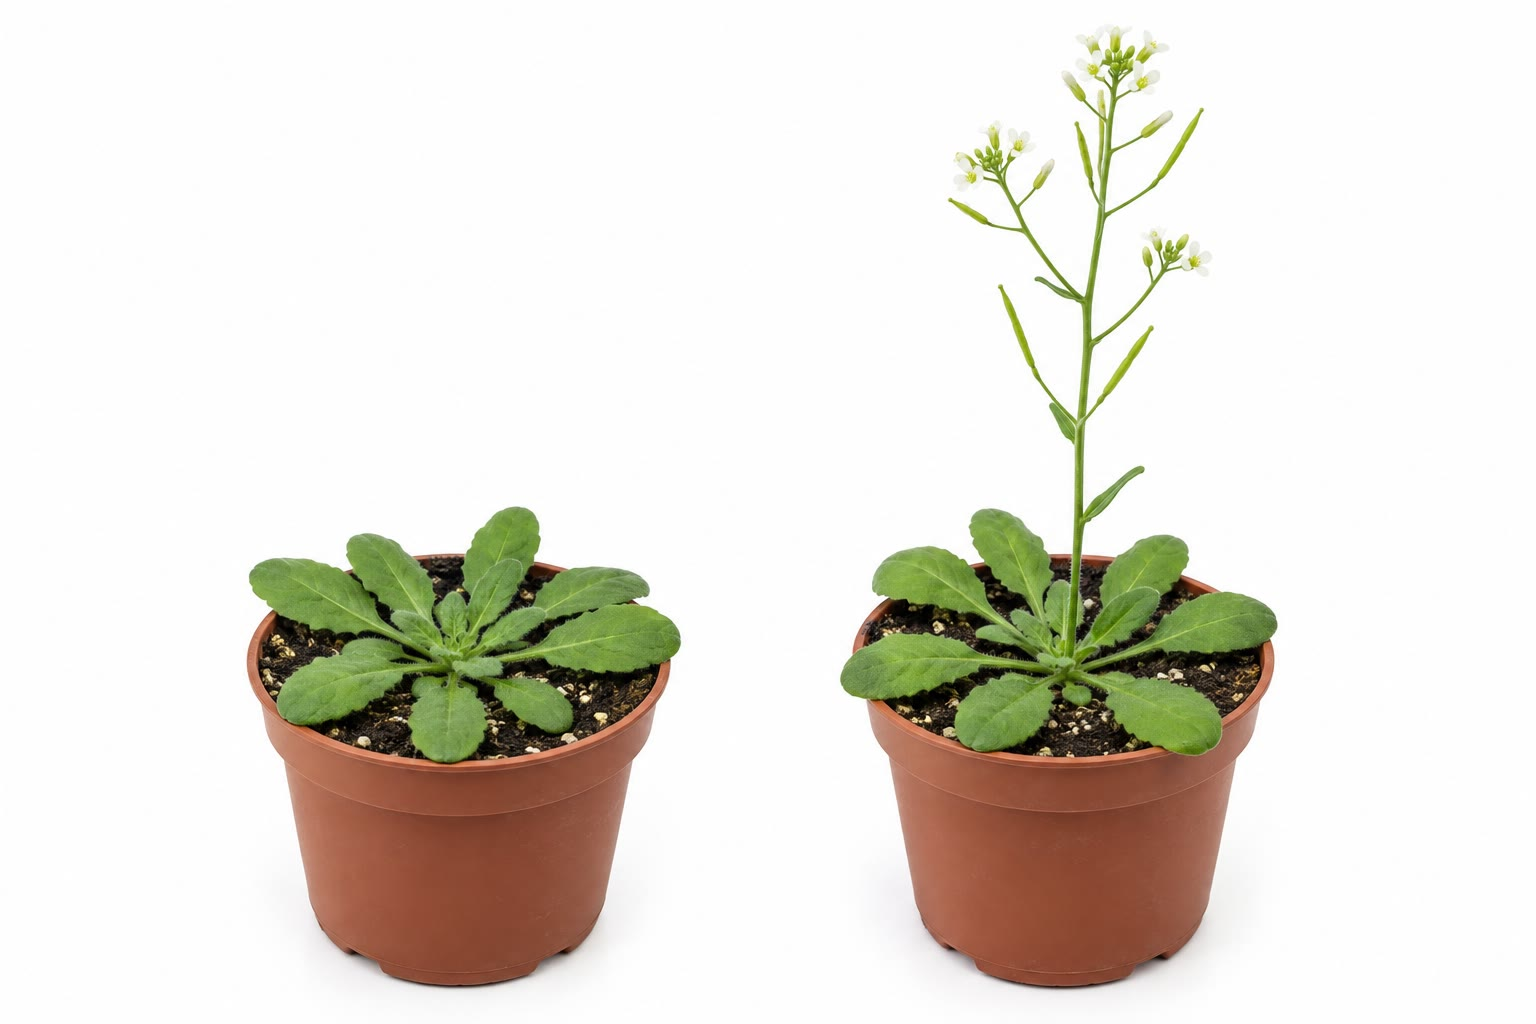
\includegraphics[width=0.58\linewidth]{images/book4/ai/b4-14-arabidopsis-daylength.jpg}

{\small \emph{Arabidopsis}, een \omterm{prop:b2:plant-flowering:photoperiod}{lange-dagplant}: in korte dagen een rozet
van bladeren; overgebracht naar lange dagen schiet ze door en bloeit ze
binnen enkele weken.}
\end{omfigure}

\begin{proposition}[Vernalisatie: de plant telt de kou]\label{prop:b2:plant-flowering:vernalisation}
\index{vernalisatie}\index{FLOWERING LOCUS C}
Wintergranen, tweejarigen (wortel, kool, vingerhoedskruid) en veel
overblijvende planten uit koude klimaten bloeien pas nadat ze weken kou
hebben meegemaakt --- \emph{vernalisatie} ---, wat ervoor zorgt dat een
plant die in de herfst kiemt op het voorjaar wacht in plaats van de vorst
in te bloeien. De kou wordt door het \omterm{def:b2:plant-meristems:meristem}{meristeem} zelf waargenomen, niet door
de bladeren; ze kan door geen enkele andere behandeling worden vervangen; en
haar effect wordt onthouden gedurende de rest van de groei van de plant,
over honderden celdelingen heen, maar niet over de \omterm{def:b2:meiosis-heredity:meiosis}{meiose} heen --- elk \omterm{def:b2:angiosperm-reproduction:seed}{zaad}
begint ongevernaliseerd. Bij \emph{Arabidopsis} is het geheugen een gen,
\emph{\omterm{prop:b2:plant-flowering:vernalisation}{FLOWERING LOCUS C}} (FLC), waarvan het product de bloei onderdrukt:
weken kou leggen het geleidelijk stil door zijn chromatine met
onderdrukkende markeringen te bedekken, het stilleggen wordt bij elke
deling gekopieerd, en het wordt in het embryo gewist. De plant
\emph{integreert} dus de kou over de tijd --- een paar koude dagen tellen
niet mee --- en een mutant zonder FLC heeft geen winter nodig.
\end{proposition}

\begin{theorem}[Waarom integratie beschermt tegen een valse lente]\label{thm:b2:plant-flowering:integration}
Stel dat een repressor met een constante snelheid $\alpha$ per koude dag
wordt stilgelegd, zodat na $n$ koude dagen de nog actieve fractie
$f_n = e^{-\alpha n}$ is, en dat bloei is toegestaan wanneer $f < f_c$.
Het vereiste aantal koude dagen is $n_c = \ln(1/f_c)/\alpha$, en
--- omdat het stilleggen stabiel is --- de koude dagen hoeven niet op
elkaar te volgen: wat telt, is hun totaal. Een plant met $n_c = 40$
dagen laat zich niet misleiden door een dooi van twee weken in januari of
door een koudeprik in oktober; een plant die alleen de huidige temperatuur
waarnam, zou in de eerste warme week bloeien. Dezelfde integratie, met een
drempel, is de manier waarop de plant de opgestapelde daglengte afleest
voordat ze zich vastlegt; beide zijn voorbeelden van een systeem dat op de
\emph{integraal} van een signaal reageert in plaats van op de ogenblikkelijke
waarde ervan.
\end{theorem}
\begin{proof}
Als elke koude dag een fractie $\alpha$ van de resterende actieve kopieën
(of van het nog ongemarkeerde chromatine) stillegt, voldoet de actieve
fractie aan $f_{n+1} = (1 - \alpha)f_n \approx e^{-\alpha}f_n$,
dus $f_n = e^{-\alpha n}$, met $n$ het aantal koude dagen; de
ongelijkheid $e^{-\alpha n} < f_c$ geeft $n > \ln(1/f_c)/\alpha$.
Dagen die niet koud zijn, tellen niet op en trekken niet af, omdat de
markeringen stabiel zijn, zodat alleen het totaal telt.
\end{proof}

\section{De bouw van de bloem: het ABC-model}

\begin{proposition}[Het ABC-model]\label{prop:b2:plant-flowering:abc}
\index{ABC-model}\index{homeotisch gen!bloem}
Een bloemmeristeem legt vier concentrische kransen aan: kelkbladen,
kroonbladen, meeldraden, \omterm{def:b2:angiosperm-reproduction:flower}{vruchtbladen}. Hun identiteit wordt bepaald door
drie klassen \emph{homeotische genen}, die in overlappende ringen werken:
klasse A alleen in krans 1 geeft kelkbladen; A en B samen in krans 2 geven
kroonbladen; B en C samen in krans 3 geven meeldraden; C alleen in krans 4
geeft \omterm{def:b2:angiosperm-reproduction:flower}{vruchtbladen}. A en C onderdrukken elkaar, zodat waar de ene verloren
gaat, de andere zich over de hele \omterm{def:b2:angiosperm-reproduction:flower}{bloem} uitbreidt. De regels voorspellen
elke enkelvoudige mutant: verlies B en de \omterm{def:b2:angiosperm-reproduction:flower}{bloem} is
kelkblad--kelkblad--vruchtblad--vruchtblad; verlies C en ze is
kelkblad--kroonblad--kroonblad--kelkblad, met daarbinnen een nieuwe \omterm{def:b2:angiosperm-reproduction:flower}{bloem},
omdat C ook het \omterm{def:b2:plant-meristems:meristem}{meristeem} stopt; verlies A en ze is
vruchtblad--meeldraad--meeldraad--vruchtblad. De meeste van deze genen
coderen voor \omterm{prop:b2:cell-differentiation:transcriptional}{transcriptiefactoren} uit één familie (MADS-box), en een vierde
klasse, E, is voor alle drie de functies nodig; B en C samen tot expressie
brengen in een blad maakt er een meeldraadachtig orgaan van. De dubbele
\omterm{def:b2:angiosperm-reproduction:flower}{bloemen} uit de tuin --- rozen, pioenen, camelia's --- zijn mutanten van
klasse C, waarvan de meeldraden extra kroonbladen zijn geworden.
\end{proposition}
\begin{proof}[Bewijsmateriaal]
Coen en Meyerowitz (1991) vergeleken de homeotische mutanten van
\emph{Arabidopsis} en van de leeuwenbek: bij beide veranderden drie klassen
\omterm{def:b2:genome-diversification:mutation}{mutaties} elk twee aangrenzende kransen, in dezelfde paren, en gedroegen de
combinaties van mutanten zich zoals het model voorspelt (de drievoudige
mutant maakt alleen bladeren). Klonering liet zien dat de genen
\omterm{prop:b2:cell-differentiation:transcriptional}{transcriptiefactoren} zijn die in de voorspelde ringen tot expressie komen;
een B-gen onder een promotor die in alle vier de kransen actief is, gaf
kroonblad--kroonblad--meeldraad--meeldraad.
\end{proof}

\begin{omfigure}
\begin{tikzpicture}[every node/.style={font=\scriptsize}]
  % four whorls as columns
  \foreach \x/\w in {0/{krans 1}, 2.2/{krans 2}, 4.4/{krans 3}, 6.6/{krans 4}} \node[above] at (\x+0.9,3.3) {\w};
  \fill[omDef!35] (0,2.4) rectangle (4.2,3.1); \node at (2.1,2.75) {A};
  \fill[omProp!40] (2.2,1.6) rectangle (6.4,2.3); \node at (4.3,1.95) {B};
  \fill[omThm!30] (4.4,0.8) rectangle (8.6,1.5); \node at (6.5,1.15) {C};
  \foreach \x/\o in {0/kelkbladen, 2.2/kroonbladen, 4.4/meeldraden, 6.6/vruchtbladen} \node[below, align=center] at (\x+0.9,0.6) {\o};
  \node[anchor=west, align=left] at (9.2,3.0) {wildtype: A, AB, BC, C};
  \node[anchor=west, align=left] at (9.2,2.3) {zonder B: kelkblad, kelkblad,\\vruchtblad, vruchtblad};
  \node[anchor=west, align=left] at (9.2,1.6) {zonder C: kelkblad, kroonblad,\\kroonblad, kelkblad\ldots};
  \node[anchor=west, align=left] at (9.2,0.9) {zonder A: vruchtblad, meeldraad,\\meeldraad, vruchtblad};
\end{tikzpicture}

{\small Het \omterm{prop:b2:plant-flowering:abc}{ABC-model}. Drie genklassen in overlappende ringen bepalen de
vier orgaanidentiteiten; het verlies van één klasse verandert twee kransen,
en de mutante \omterm{def:b2:angiosperm-reproduction:flower}{bloemen} zijn precies die welke worden voorspeld.}
\end{omfigure}

\begin{omfigure}
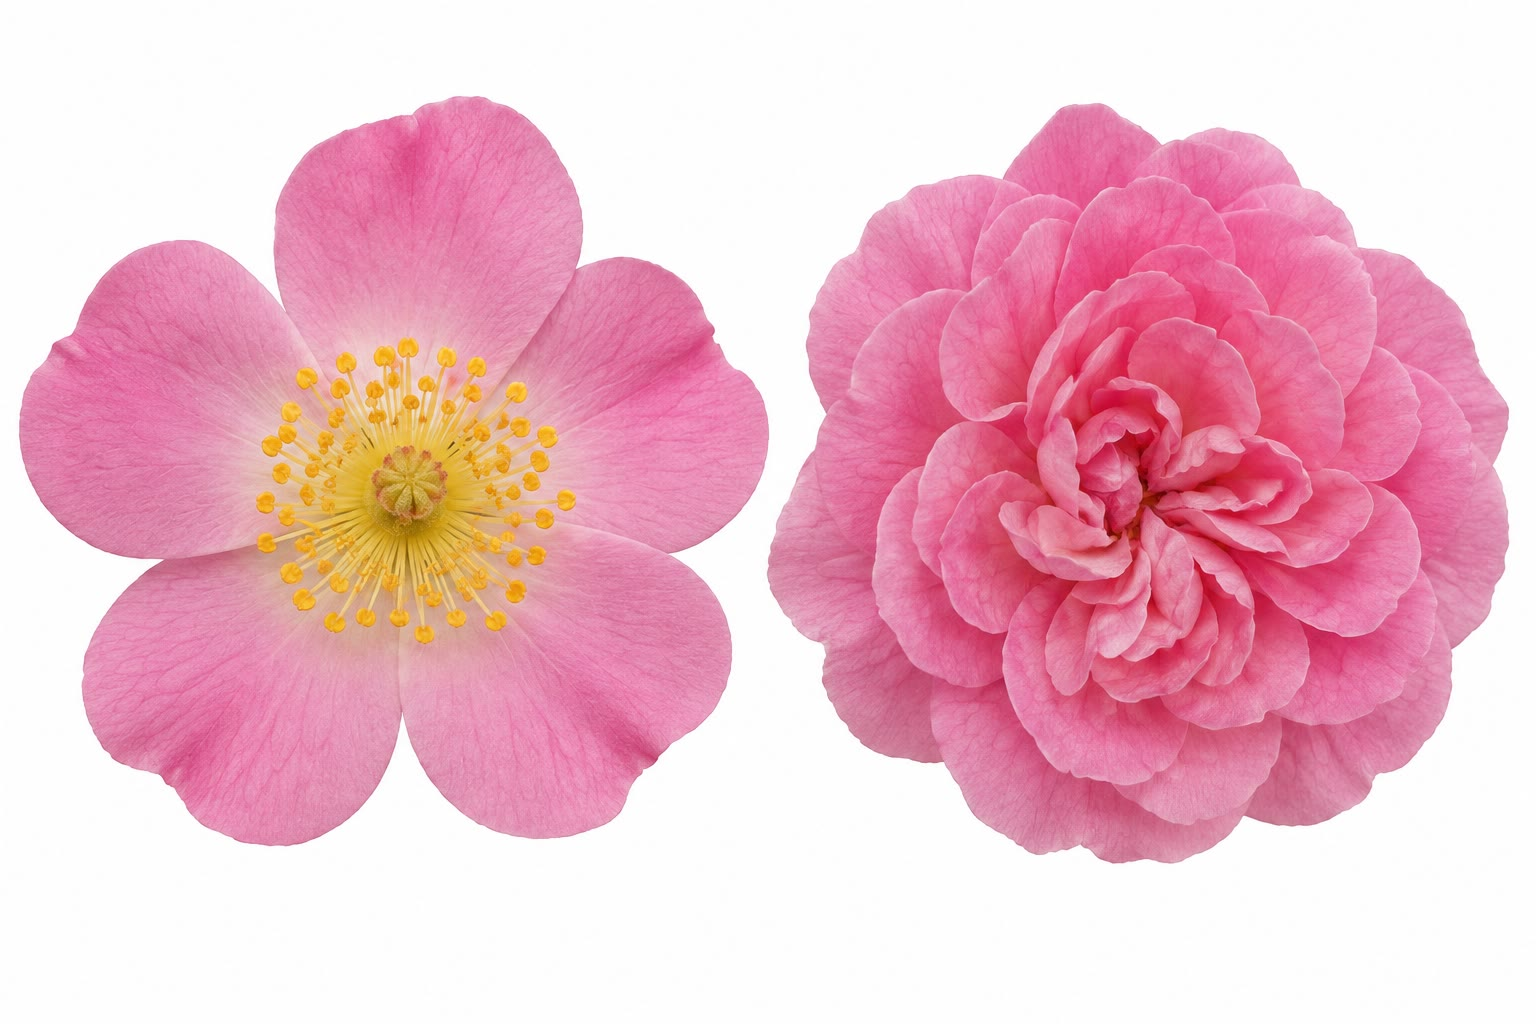
\includegraphics[width=0.58\linewidth]{images/book4/ai/b4-14-double-flower.jpg}

{\small Een wildtype \omterm{def:b2:angiosperm-reproduction:flower}{bloem} naast een dubbele vorm: de meeldraden zijn
kroonbladen geworden --- een mutant van klasse C, al eeuwenlang door tuiniers
geselecteerd voordat iemand wist waarom hij dubbel was.}
\end{omfigure}

\section{Kiemrust en kieming}

\begin{definition}[Kiemrust van zaden]\label{def:b2:plant-flowering:dormancy}
\index{kiemrust!zaad}\index{abscisinezuur}\index{gibberelline}\index{stratificatie}
Een levensvatbaar \omterm{def:b2:angiosperm-reproduction:seed}{zaad} dat niet kiemt onder omstandigheden die groei zouden
toelaten, is \emph{in \omterm{def:b2:angiosperm-reproduction:seed}{kiemrust}}. De \omterm{def:b2:angiosperm-reproduction:seed}{kiemrust} wordt tijdens de rijping van
het \omterm{def:b2:angiosperm-reproduction:seed}{zaad} opgelegd door \emph{abscisinezuur} (ABA), dat ook de opslag van
reserves en het uitdrogen van het embryo aanstuurt, en ze wordt in stand
gehouden door de \omterm{def:b2:angiosperm-reproduction:seed}{zaadhuid} (ondoorlaatbaar voor water of zuurstof, mechanisch
remmend) of door de eigen toestand van het embryo. Ze wordt doorbroken door
de signalen die het einde van het ongunstige seizoen markeren: weken kou en
vocht (\emph{stratificatie}, de vernalisatie van het \omterm{def:b2:angiosperm-reproduction:seed}{zaad}), licht --- voor
kleine zaden die dicht bij het oppervlak moeten liggen, waargenomen door
fytochroom --- of duisternis, wisselende temperaturen, het uitspoelen van
remstoffen door regen, het opruwen van de \omterm{def:b2:angiosperm-reproduction:seed}{zaadhuid} door de bodem of een
darm, rook en hitte na een brand. De beslissing is een evenwicht tussen ABA
en \emph{gibberelline}: de doorbrekende signalen verlagen ABA en verhogen
gibberelline, dat de reserves mobiliseert
(\cref{ch:b2:angiosperm-reproduction}) en de kiemwortel laat groeien. Een
populatie zaden is niet uniform: een deel kiemt bij de eerste gelegenheid,
de rest wacht een jaar of langer, zodat geen enkel slecht seizoen het hele
cohort doodt --- de \emph{zaadbank}, een verzekering tegen een
onvoorspelbare wereld.
\end{definition}
\begin{proof}[Bewijsmateriaal]
Slazaden (Borthwick, 1952) kiemen in het donker na een flits rood licht en
niet na een flits verrood; krijgen ze rood, dan verrood, dan rood, dan
kiemen ze --- de laatste flits beslist. Hetzelfde omkeerbare pigment dat de
bloei timet, zet de kieming in gang. Zaden van veel bomen die vers in warme
grond worden gezaaid, doen niets; dezelfde zaden kiemen na twee maanden in
een vochtige koelkast meteen, en ABA-deficiënte mutanten kiemen al op de
plant, voordat het \omterm{def:b2:angiosperm-reproduction:seed}{zaad} zelfs maar droog is.
\end{proof}

\begin{omfigure}
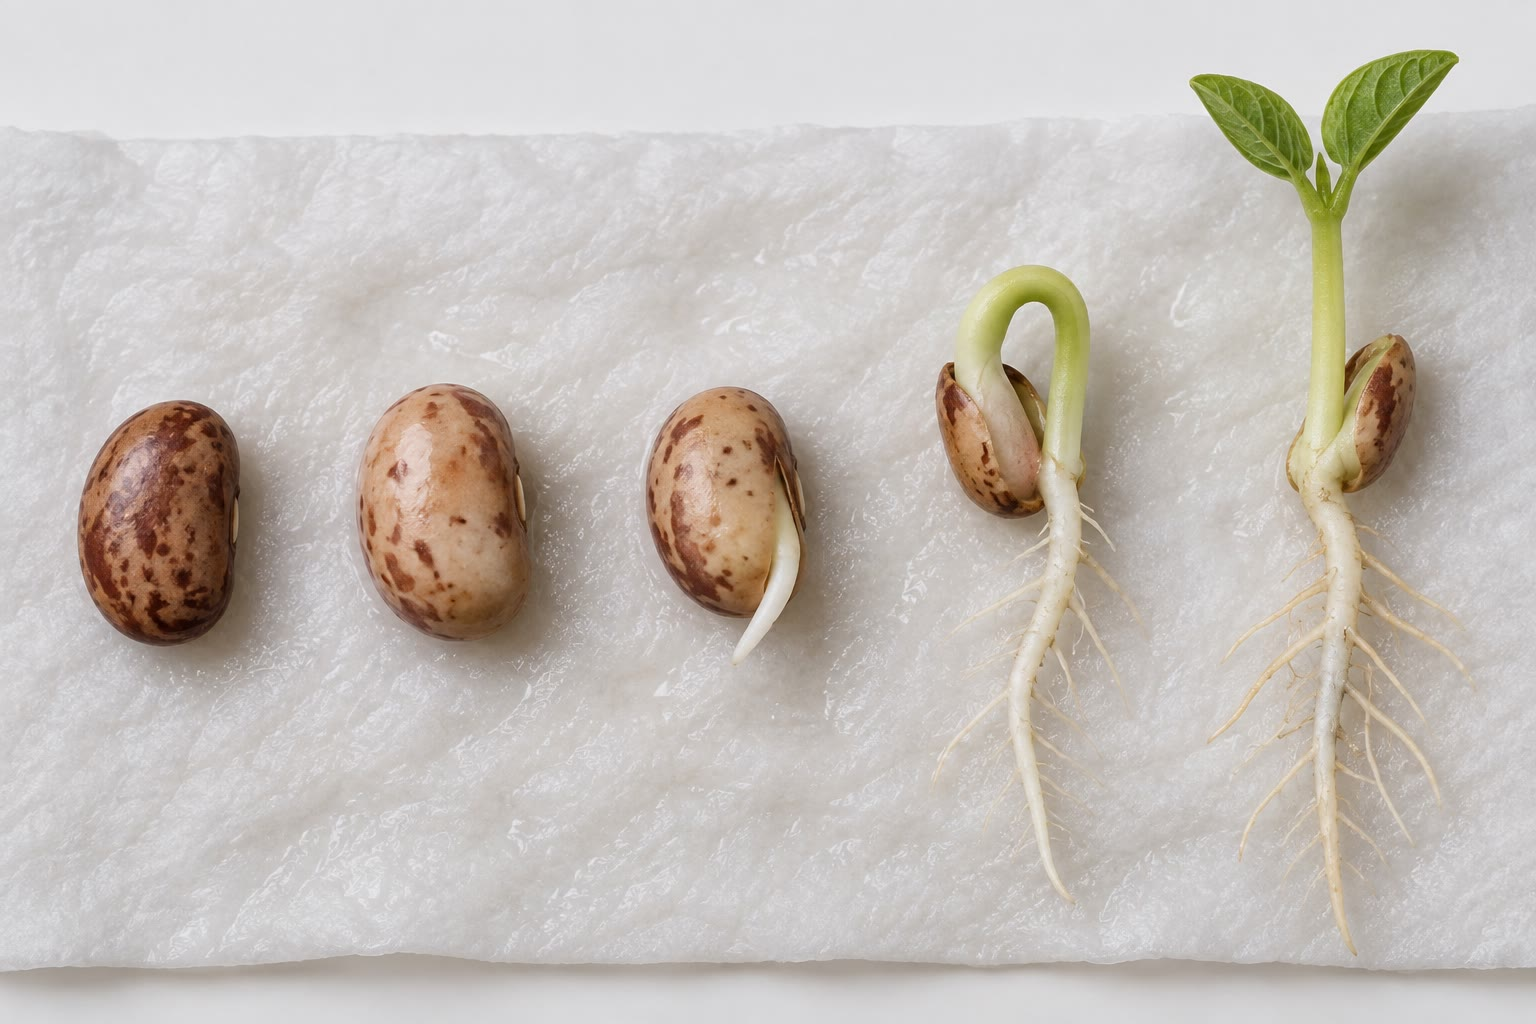
\includegraphics[width=0.66\linewidth]{images/book4/ai/b4-14-germinating-beans.jpg}

{\small Kieming van een boon: het \omterm{def:b2:angiosperm-reproduction:seed}{zaad} neemt water op, de kiemwortel
verschijnt eerst, het hypocotyl duwt zich als een haak omhoog door de grond,
en de haak strekt zich in het licht terwijl de eerste bladeren opengaan.}
\end{omfigure}

\begin{theorem}[Kiemen als weddenschap]\label{thm:b2:plant-flowering:bet}
\index{risicospreiding}
Laat een fractie $g$ van een cohort zaden elk jaar kiemen en de rest met
kans $s$ in de bodem tot het volgende jaar overleven. In een goed jaar
laat een kiemend \omterm{def:b2:angiosperm-reproduction:seed}{zaad} $R_g$ zaden na; in een slecht jaar geen enkel; jaren
zijn goed met kans $p$. Een strategie die alles in één keer laat kiemen
($g = 1$) heeft over een reeks jaren een groeisnelheid op lange termijn,
met $\ln$ gemiddeld, van $p\ln R_g + (1 - p)\ln 0 =
-\infty$: één slecht jaar dooft haar uit. Een strategie met $g < 1$
groeit in goede jaren met een factor $gR_g + (1 - g)s$ en in slechte jaren
met $(1 - g)s > 0$, zodat haar groeisnelheid op lange termijn,
\[
r = p\ln\bigl(gR_g + (1 - g)s\bigr) + (1 - p)\ln\bigl((1 - g)s\bigr),
\]
eindig is en, voor $p$ niet te dicht bij 1, maximaal is bij een
tussenliggende $g$. Met $R_g = 20$, $s = 0.8$ en $p = 0.7$ ligt het
optimum bij ongeveer $g = 0.7$: laat het meeste kiemen, houd een reserve.
\omterm{def:b2:angiosperm-reproduction:seed}{Kiemrust} is geen falen om te kiemen, maar een geëvolueerde gedeeltelijke
weigering.
\end{theorem}
\begin{proof}
De populatiegrootte na $T$ jaar is het product van de jaarlijkse factoren,
zodat de groeisnelheid het gemiddelde van hun logaritmen is (de
meetkundig gemiddelde snelheid), en die maximaliseert selectie over lange
reeksen. Met $g = 1$ is de factor in een slecht jaar nul en de logaritme
$-\infty$. Voor $g < 1$ zijn beide factoren positief; differentiëren van
$r$ naar $g$ en de afgeleide nul stellen geeft het optimum, dat voor de
genoemde waarden bij ongeveer $g = 0.7$ ligt (evaluatie van $r$ bij
$g = 0.4, 0.6, 0.8, 1$ geeft $1.28$, $1.42$,
$1.40$, $-\infty$).
\end{proof}

\begin{omfigure}
\begin{tikzpicture}
\begin{axis}[
  width=0.7\linewidth, height=5.4cm,
  axis x line=bottom, axis y line=left,
  xmin=0, xmax=1, ymin=0, ymax=1.7,
  xlabel={fractie die elk jaar kiemt, $g$}, ylabel={groeisnelheid op lange termijn $r$},
  xlabel style={font=\small, at={(axis description cs:0.5,-0.13)}, anchor=north},
  ylabel style={font=\small},
  tick label style={font=\small}, xtick={0,0.2,0.4,0.6,0.8,1}, ytick={0,0.5,1,1.5},
  clip=false,
]
\addplot[very thick, omDef, domain=0.02:0.97, samples=100] {0.7*ln(20*x + 0.8*(1-x)) + 0.3*ln(0.8*(1-x))};
\draw[dashed, gray] (axis cs:0.7,0) -- (axis cs:0.7,1.43);
\node[font=\scriptsize, anchor=south] at (axis cs:0.7,1.45) {optimum: houd \qty{30}{\%} in de bodem};
\node[font=\scriptsize, anchor=north west, align=left] at (axis cs:0.7,0.6) {$g \to 1$: één slecht jaar\\vaagt het cohort weg};
\end{axis}
\end{tikzpicture}

{\small \omterm{thm:b2:plant-flowering:bet}{Risicospreiding} door \omterm{def:b2:angiosperm-reproduction:seed}{kiemrust}. Met zeven goede jaren op tien wordt
een cohort dat helemaal kiemt, uiteindelijk door een slecht jaar vernietigd;
een cohort dat een deel van zijn zaden achterhoudt, groeit op lange termijn
het snelst.}
\end{omfigure}

\section{Opgaven}

\begin{exercise}[$\star$]\label{exo:b2:plant-flowering:1}
Onderscheid vegetatieve meristemen, bloeiwijzemeristemen en bloemmeristemen,
en zeg welke begrensd zijn.
\end{exercise}

\begin{exercise}[$\star$]\label{exo:b2:plant-flowering:2}
Definieer \omterm{prop:b2:plant-flowering:photoperiod}{korte-dagplanten}, \omterm{prop:b2:plant-flowering:photoperiod}{lange-dagplanten} en dagneutrale planten met bij
elk een voorbeeld, en zeg wat een \omterm{prop:b2:plant-flowering:photoperiod}{korte-dagplant} eigenlijk meet.
\end{exercise}

\begin{exercise}[$\star$]\label{exo:b2:plant-flowering:3}
Geef de orgaanidentiteit van elke krans in het wildtype en in de drie
enkelvoudige mutanten van het \omterm{prop:b2:plant-flowering:abc}{ABC-model}.
\end{exercise}

\begin{exercise}[$\star$]\label{exo:b2:plant-flowering:4}
Noem vier signalen die de \omterm{def:b2:angiosperm-reproduction:seed}{kiemrust} van zaden doorbreken en, bij elk, het
seizoen of de plaats die het meldt.
\end{exercise}

\begin{exercise}[$\star\star$]\label{exo:b2:plant-flowering:5}
Een \omterm{prop:b2:plant-flowering:photoperiod}{korte-dagplant} heeft een kritische nacht van \qty{10}{h}. Zeg of ze
bloeit onder: \qty{16}{h} licht/\qty{8}{h} donker; \qty{12}{h}/\qty{12}{h};
\qty{12}{h} licht, \qty{6}{h} donker, één minuut licht, \qty{6}{h} donker;
\qty{8}{h} licht, \qty{4}{h} donker, \qty{4}{h} licht, \qty{8}{h} donker.
\end{exercise}

\begin{exercise}[$\star\star$]\label{exo:b2:plant-flowering:6}
Een blad van een geïnduceerde \omterm{prop:b2:plant-flowering:photoperiod}{korte-dagplant} wordt geënt op een
\omterm{prop:b2:plant-flowering:photoperiod}{lange-dagplant} die in lange dagen wordt gehouden, en de \omterm{prop:b2:plant-flowering:photoperiod}{lange-dagplant}
bloeit. Wat toont dit aan over \omterm{def:b2:plant-flowering:florigen}{florigeen}? En als de ent wordt gemaakt met
een blad dat wel geïnduceerd is, maar waarvan het floëem in de bladsteel is
onderbroken?
\end{exercise}

\begin{exercise}[$\star\star$]\label{exo:b2:plant-flowering:7}
Kou legt de repressor stil met $\alpha = 0.05$ per dag en de bloei vereist
$f < 0.15$. Hoeveel koude dagen zijn er nodig? Een winter heeft drie koude
periodes van 15, 12 en 20 dagen, gescheiden door dooi: is de plant
gevernaliseerd? En als $\alpha$ gelijk was aan $0.02$?
\end{exercise}

\begin{exercise}[$\star\star$]\label{exo:b2:plant-flowering:8}
Leg in termen van chromatine uit waarom het geheugen van een gevernaliseerde
plant in haar zaden verloren gaat, en waarom dat nuttig is.
\end{exercise}

\begin{exercise}[$\star\star$]\label{exo:b2:plant-flowering:9}
Slazaden krijgen in het donker de reeksen: R; R dan VR; R, VR, R; R, VR, R,
VR. Voorspel de kieming in elk geval en leg die uit in termen van de twee
vormen van fytochroom.
\end{exercise}

\begin{exercise}[$\star\star\star$]\label{exo:b2:plant-flowering:10}
Bereken in het model van de \omterm{thm:b2:plant-flowering:bet}{risicospreiding} met $R_g = 20$ en $s = 0.8$ de
groeisnelheid op lange termijn voor $g = 0.4$, $0.6$, $0.8$ en $1$ bij
$p = 0.7$, en opnieuw bij $p = 0.95$. Hoe verschuift het optimum, en wat
voorspelt dat voor woestijnen tegenover weilanden?
\end{exercise}

\begin{exercise}[$\star\star\star$]\label{exo:b2:plant-flowering:11}
Voorspel de \omterm{def:b2:angiosperm-reproduction:flower}{bloem} die ontstaat wanneer een gen van klasse B in alle vier de
kransen tot expressie wordt gebracht; wanneer klasse C in alle vier tot
expressie komt; bij een dubbelmutant zonder A en B. Leg daarna uit waarom de
\omterm{def:b2:angiosperm-reproduction:flower}{bloem} zonder C kransen blijft maken.
\end{exercise}

\begin{exercise}[$\star\star\star$]\label{exo:b2:plant-flowering:12}
``Een plant beslist te bloeien door signalen te integreren die ze niet kan
sturen.'' Bespreek de drie integraties van dit hoofdstuk --- van de
daglengte, van de kou, van de jaren in de zaadbank --- en waartegen een
integrator de plant beschermt, wat een eenvoudige drempel niet zou doen.
\end{exercise}

\section{Vraagstuk: de kalender van de kweker}

\begin{problem}[{Weekendvraagstuk --- een chrysantenkweker plant de bloei
met lampen, een tarweveredelaar telt kou, de dubbele bloem van een bloemist
wordt verklaard, en de kiemrust van een partij zaden wordt gemodelleerd,
met als besluit de nachtlengte die het gewas in bloei zet, de koude dagen
die de tarwe nodig heeft, en de beste kiemfractie}]
\label{pb:b2:plant-flowering:1}
De chrysant is een \omterm{prop:b2:plant-flowering:photoperiod}{korte-dagplant} met een kritische nachtlengte van
\qty{9.5}{h}; de inductie vereist \num{12} opeenvolgende inductieve
nachten, en de \omterm{def:b2:angiosperm-reproduction:flower}{bloemen} gaan \num{8} weken na de inductie open. In november
is de kas donker van 17:00 tot 07:30. Wintertarwe
heeft $\alpha = 0.06$ per koude dag en bloeit wanneer $f < 0.10$. Partij
zaden: $R_g = 15$, $s = 0.7$, goede jaren met kans $p$.

\medskip
\noindent\textbf{Deel I --- De kas.}
\begin{enumerate}
  \item In juni duurt de natuurlijke nacht \qty{8}{h}. Zal het gewas
        bloeien? Wat moet de kweker doen om in augustus \omterm{def:b2:angiosperm-reproduction:flower}{bloemen} te verkopen?
  \item De kweker bedekt het gewas van 19:00 tot 07:00 met zwart doek. Welke
        nachtlengte ziet de plant, en wanneer moet het bedekken beginnen voor
        een bloei op 15~augustus?
  \item In november duurt de natuurlijke nacht \qty{14}{h} en wil de kweker
        de bloei tot Kerstmis \emph{uitstellen}. Stel een belichtingsschema
        voor en leg uit waarom een korte flits volstaat.
  \item De flits wordt om 21:00 gegeven in plaats van om 00:00, en de
        inductie wordt niet voorkomen. Verklaar dit met de kritische
        nachtlengte.
  \item In één nacht van de twaalf blijft het doek eraf. Voorspel wat er
        gebeurt, en zeg wat een stekelnoot zou hebben gedaan.
  \item De flits wordt in groen licht gegeven en werkt niet; in rood licht
        werkt hij wel; rood gevolgd door verrood werkt niet. Verklaar.
  \item Eén blad van een geïnduceerde plant wordt geënt op een plant onder
        lange dagen. Voorspel wat er gebeurt, en zeg wat dit identificeert.
\end{enumerate}

\medskip
\noindent\textbf{Deel II --- De tarwe.}
\begin{enumerate}[resume]
  \item Hoeveel koude dagen heeft de tarwe nodig?
  \item In oktober gezaaid krijgt ze 10 koude dagen in november, een zachte
        december, 25 in januari en 12 in februari. Wanneer is ze
        gevernaliseerd?
  \item In maart gezaaid krijgt ze 6 koude dagen. Bloeit ze die zomer? Wat
        is het gevolg voor de landbouw?
  \item Een mutant mist de repressor. Voorspel zijn gedrag en zeg waarom
        veredelaars zulke tarwes ``zomertarwes'' noemen.
  \item Leg uit waarom het geheugen van de kou de delingen van het \omterm{def:b2:plant-meristems:meristem}{meristeem}
        in het voorjaar overleeft, maar niet de \omterm{def:b2:meiosis-heredity:meiosis}{meiose} die de volgende
        generatie maakt.
  \item Waarom moet de kou in het \omterm{def:b2:plant-meristems:meristem}{meristeem} worden geteld en niet in de
        bladeren, anders dan de daglengte?
\end{enumerate}

\medskip
\noindent\textbf{Deel III --- De bloemist.}
\begin{enumerate}[resume]
  \item Een dubbele roos heeft kroonbladen waar de meeldraden zouden moeten
        zitten en enkele extra kroonbladen in het midden. Welke genklasse is
        uitgevallen? Geef de kransformule.
  \item Zulke rozen zijn steriel als stuifmeelouder, maar zetten soms \omterm{def:b2:angiosperm-reproduction:seed}{zaad}.
        Verklaar beide feiten met het \omterm{prop:b2:plant-flowering:abc}{ABC-model}.
  \item Een leeuwenbek heeft meeldraden in plaats van kroonbladen en
        \omterm{def:b2:angiosperm-reproduction:flower}{vruchtbladen} in plaats van kelkbladen. Welke klasse is uitgevallen?
  \item Voorspel de \omterm{def:b2:angiosperm-reproduction:flower}{bloem} van een plant waarin klasse C naast zijn normale
        kransen ook in krans 1 tot expressie komt.
  \item Waarom gaven dezelfde \omterm{def:b2:genome-diversification:mutation}{mutaties} dezelfde omvormingen bij een roos,
        een leeuwenbek en \emph{Arabidopsis}, planten die honderd miljoen jaar
        uit elkaar liggen?
  \item In krans 2 van een wildtype \omterm{def:b2:angiosperm-reproduction:flower}{bloem} zijn zowel A als B actief.
        Voorspel het orgaan als daar alleen B actief was.
\end{enumerate}

\medskip
\noindent\textbf{Deel IV --- De partij zaden.}
\begin{enumerate}[resume]
  \item Bereken de groeisnelheid op lange termijn $r$ voor $g = 0.5$, $0.7$
        en $0.9$ bij $p = 0.8$.
  \item Welke van de drie is de beste? Wat gebeurt er bij $g = 1$?
  \item Bereken opnieuw voor $p = 0.5$ (een woestijn). Welke $g$ is nu de
        beste?
  \item Een teler zaait de hele partij in een goed jaar op één veld en oogst
        $R_g$ per \omterm{def:b2:angiosperm-reproduction:seed}{zaad}. Leg uit waarom zijn strategie verschilt van die van
        de plant en wat hij moet doen om het ras door een slecht jaar heen te
        behouden.
  \item De zaden hebben licht nodig om te kiemen. Leg de adaptieve zin
        hiervan uit voor een klein \omterm{def:b2:angiosperm-reproduction:seed}{zaad}, en voorspel wat ploegen met de
        zaadbank doet.
  \item Formuleer het resultaat: de kritische nachtlengte en het schema van
        het bedekken, de koudebehoefte van de tarwe, en de beste $g$ voor
        $p = 0.8$ en $p = 0.5$.
\end{enumerate}
\end{problem}
